\section{Experimental Setup}
\label{sec:setup}

This section describes the data, the two splits, the comparison models, the tuning and the rule used to compare methods.
The duplicate review, background audit, label check and heat-map ratings were done by disclosed AI model raters; one of
the two leaf-width measurers was also an AI model.

\subsection{Data}
\label{sec:setup:data}
The primary data are the labelled photos of the Rice Diseases Image Dataset \cite{do2019} (MIT licence; Kaggle release last updated 2019-11-15, downloaded on
2026-09-26): 3{,}355 photos of healthy leaves (1{,}488), leaf blast (779), brown spot (523) and hispa (565), with shorter
sides of 734--3{,}120 px (Fig.~\ref{fig:samples}). The download holds two more hispa photos than the published count (563). Three phone cameras
appear, and hispa photos all come from one of them.
A two-stage check (perceptual hash or embedding similarity, then a keypoint match) flagged near-duplicates, and two model
raters reviewed the candidates (Cohen's $\kappa$ \cite{cohen1960kappa} of 0.77; the 61 disagreements were adjudicated
and both original verdicts were kept). It confirmed 349 same-leaf pairs. Twenty-one photos that appear under
two different labels were excluded, which leaves 3{,}334 photos in 3{,}045 near-duplicate groups for all experiments.
A background audit of 240 photos (60 per class) found every background plain, and a label check of 80 photos
found one that looked like another class; no label was changed.

The leaf-scale rule rests on a pixel-scale audit. We measured leaf width on 30 photos spread over the size range (29 were
measurable). Width and shorter side correlated with Spearman $\rho=0.539$, above the pre-declared threshold of 0.5, so
photos are rescaled. The audit is borderline: leave-one-out correlations run from 0.488 to 0.613. The two measurers
agreed closely ($\rho=0.978$).

Paddy Doctor \cite{petchiammal2023} (full release from IEEE DataPort, DOI 10.21227/hz4v-af08; CC BY 4.0; downloaded on 2026-09-26) has 16{,}225 field photos of $1080\times1440$ px
in 13 classes. Its four classes shared with the primary data hold 8{,}086 photos once 78 byte-identical copies are
removed; none matches a primary photo. It was used only for zero-shot scoring, never for training, tuning or selection. A
224-px tile covers about three times more leaf on Paddy Doctor photos than on rescaled primary photos (median leaf width
194.9 against 64.5 px; the second value is a model-rater estimate from 30 photos of the nine classes we did not test).
We therefore scored three zoom levels: native, in which the photo is tiled as stored and which was fixed in advance as the
headline; midway ($\times1.73$); and matched ($\times3.0$).

\begin{figure}[t]
\centering
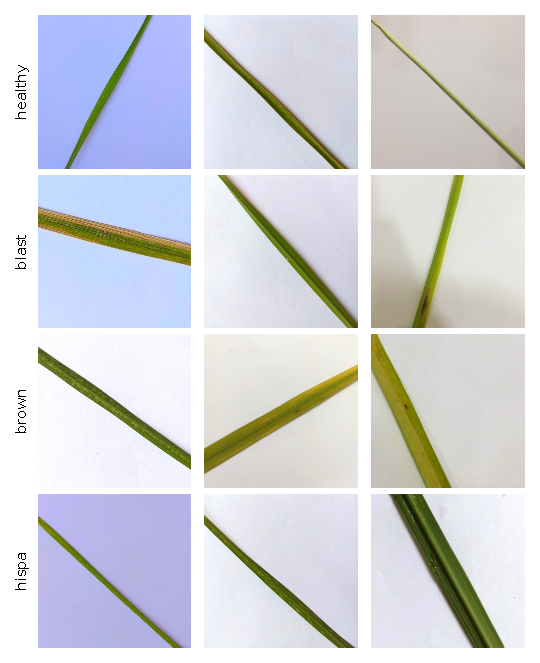
\includegraphics[width=0.6\columnwidth]{final_samples.pdf}
\caption{Example photos of the primary dataset: three per class (rows: healthy, leaf blast, brown spot, hispa).}
\label{fig:samples}
\end{figure}

\subsection{Splits}
\label{sec:setup:splits}
Each split was made once, before any model was trained on it, and is never regenerated; the locked split was made before any other processing. The \emph{locked split} is a stratified,
near-duplicate-grouped five-fold split (seed 2026). In each round one fold is the test set, and a stratified, grouped
$1/8$ of the rest is validation, giving about 70\,\%, 10\,\% and 20\,\% of the photos. Because photos were shot in
long sessions, it still lets a test photo have a training photo of the same camera a few seconds away (90.2\,\% of test
photos within 10 s). The \emph{session-blocked split} therefore keeps whole capture blocks (runs of photos of one camera
with no pause over 60 s; 74 blocks, the largest holding 287 photos) on one side: no test photo has a same-camera training photo within 60 s. It uses the same folds procedure
and the same validation rule. Block sizes make class shares uneven across rounds (worst deviation 26.5 points); they are
reported, not enforced. Test sets hold 616--738 photos. The session-blocked split was declared after the locked-split test
results were seen, and every method was then tuned again on its validation photos; it is the headline split, and the
locked split is the secondary one. Augmented copies stay in the role of their source photo and never reach validation or
test, which automated tests enforce.

\subsection{Comparison models}
Four ImageNet-pretrained models were fine-tuned on whole photos, padded to a square and resized:
InceptionV3 \cite{szegedy2016inception}, EfficientNetV2-S \cite{tan2021efficientnetv2}, ConvNeXt-T \cite{liu2022convnext}
and Swin-T \cite{liu2021swin}, at 224 px; at 128 px; at 224 px after Otsu background removal; and, for ConvNeXt-T, which
had the best validation score at 224 px, at 448 px. Linear probes at 224 and 512 px fit class-balanced
logistic regression on one frozen DINOv3 description of the whole photo. Six controls see no leaf shape: majority class, random by class
share, colour only, background only, file properties only and camera only; a seventh predicts the class of the nearest
training photo in time from the same camera.

\subsection{Training and selection}
\label{sec:setup:training}
All trained models used inverse-frequency class weights and cross-entropy with label smoothing 0.1
\cite{muller2019labelsmoothing}; we generate no images. Training photos were augmented with random resized crops, flips,
rotations and colour changes. Fine-tuning used AdamW \cite{loshchilov2019adamw} with weight decay 0.05, two warm-up epochs
and a cosine decay \cite{loshchilov2017sgdr}, mixed precision \cite{micikevicius2018mixed}, batches of 32, at most 40
epochs and patience 8 on validation macro-F1. For each architecture three learning rates ($3\times10^{-5}$, $10^{-4}$,
$3\times10^{-4}$) were tried in all five rounds, and the grid was extended by at most three further values when the best was
at an edge. Each aggregator head (attention, mean, max, and the whole-photo head) received 40 Optuna trials
\cite{akiba2019optuna} per study over learning rate, weight decay, projection width, dropout, tile dropout and descriptor,
in two studies with different learning-rate ranges, and kept the better; the probes searched six L2 strengths. Every
choice used the mean validation macro-F1 over the five rounds. Budgets match within a method family and differ across
families. Models were trained with PyTorch \cite{paszke2019pytorch}, timm \cite{wightman2019timm}, Transformers
\cite{wolf2020transformers} and scikit-learn \cite{pedregosa2011sklearn}, on an RTX 4060 (8\,GB) with a Ryzen 7 7700 and
16\,GB of RAM; some description caches were built on Kaggle T4 GPUs or a second PC (each cache on one machine). Every run
record keeps the configuration, code commit, split checksum, and per-photo predictions.

\subsection{Metrics and the comparison rule}
\label{sec:setup:metrics}
The main metric is macro-F1, the mean over the four classes of the F1 score, with balanced accuracy (the mean recall). We also
report per-class recall, confusion matrices (from which per-class precision follows; Table~\ref{tab:final_confusion}) and the expected calibration error (ECE, 15 equal-width bins
\cite{guo2017calibration}). Every table gives the mean $\pm$ SD over the five test rounds; there is one training seed per
round, so the SD measures variation over folds, not over seeds; the model trained in a round is its ``round-model''. Differences between two methods are computed on the
pooled test predictions (every photo once) and come with two 95\,\% percentile bootstrap ranges \cite{efron1993bootstrap}:
the \emph{photo range} resamples photos (2{,}000 class-stratified resamples) and the \emph{block range} resamples whole
capture blocks, and is wider when neighbouring photos look alike. ``A beats B'' requires the range of the difference to lie
above zero \emph{and} A to win at least four of the five rounds (a tied round is won by neither); we state the verdict
under both ranges, and otherwise write ``no clear difference''. Plain accuracy is kept in every run record. Each frozen configuration was evaluated on test once.
Comparisons declared after the means were seen are marked as such where they are reported.
